\documentclass[conference]{IEEEtran}
\IEEEoverridecommandlockouts
\usepackage[T1]{fontenc}
\usepackage{cite}
\usepackage{amsmath,amssymb}
\usepackage{graphicx}
\usepackage{array}
\usepackage{url}
\usepackage[hidelinks]{hyperref}
\graphicspath{{figures/}}
\begin{document}
\title{CogniFin Coach: A Cognitive-Profile-Aware Financial Decision Coach with Bayesian Bias Modelling and Self-Report Grounding}
\author{\IEEEauthorblockN{Aung Khine Moe}\IEEEauthorblockA{\textit{Department of Computer Engineering} \\ \textit{King Mongkut's University of Technology Thonburi}\\ Bangkok, Thailand \\ Student ID: 68070701715 \quad aung.moe1@kmutt.ac.th}}
\maketitle
\begin{abstract}
Retail investors repeat the same emotionally driven mistakes---selling in a panic after a drop, chasing a rally, over-concentrating, or riding losers---even when they know the textbook advice, and generic financial education rarely changes this behaviour. We present CogniFin Coach, a cognitive computing system that couples a dual-layer user model with grounded natural-language coaching inside a turn-based investing simulation on synthetic prices. A 15-item quiz supplies a prior over four bias traits (loss aversion, overconfidence, herding/FOMO, panic selling); a perception layer converts each decision into six behavioural events and three opportunity contexts; a long-term layer maintains a Beta--Bernoulli belief per trait that is updated from fired-versus-resisted opportunities, while a short-term layer tracks drawdown stress and decision speed as a System-1 proxy. A mismatch detector, motivated by the bias blind spot, contrasts what users claimed with what they did. A large language model writes the coaching message behind a validator and an offline fallback, whereas the ``Why this?'' explanation---evidence, mechanism, estimate \ensuremath{\pm} uncertainty and citation---is assembled deterministically from a knowledge base so it cannot hallucinate. In an evaluation with 300 simulated personas, the Bayesian update matched or improved quiz-only top-trait accuracy (0.797 vs. 0.790; 0.730 vs. 0.717 under an under-reporting quiz), whereas a naive additive rule degraded it (0.720; 0.657); the mismatch detector reached 0.91 recall at 0.64 precision; and personalised messages cited the user's own numbers, unlike rule templates. We discuss why simulated results bound, rather than establish, efficacy for people.
\end{abstract}
\begin{IEEEkeywords}
cognitive computing, user modelling, behavioural finance, cognitive biases, Bayesian inference, large language models, explainable AI, debiasing
\end{IEEEkeywords}

\section{Introduction}
Individual investors lose money in systematic, predictable ways. Households that trade the most earn the lowest net returns~\cite{bo00}, investors realise gains far more readily than losses~\cite{ss85,odean98}, and sharp market falls trigger sales that lock in losses just before recoveries. These patterns are not primarily failures of knowledge: a meta-analysis of 168 studies found that financial-literacy interventions explain only about 0.1\% of the variance in downstream financial behaviour, and that the effect decays within months~\cite{flm14}, even though literacy itself matters for outcomes~\cite{lm14}. Robo-advisers can reduce some behavioural biases, but they do so largely by taking the decision away from the investor rather than helping the investor understand it~\cite{dpr19}.

Cognitive science suggests why. Under time pressure and loss, fast intuitive (System-1) processing and visceral states dominate slower deliberation~\cite{kahneman11,es13,loewenstein96}, and people readily see biases in others but not in themselves---the \textit{bias blind spot}~\cite{pronin02}. Debiasing work shows that feedback which is timely, specific and tied to the person's own decision can reduce biased judgement, sometimes durably~\cite{fischhoff82,larrick04,morewedge15}. A coach that helps therefore has to (i) \textit{perceive} decisions as they happen, (ii) maintain a \textit{model of the user} that combines self-report with behavioural evidence and knows how uncertain it is, (iii) \textit{reason} about which bias plausibly drove a decision, and (iv) \textit{explain} that inference transparently enough to support the user's own metacognitive monitoring~\cite{flavell79}.

This paper describes CogniFin Coach, a prototype that implements these four capabilities in a closed perception--action loop and evaluates each one. We ask four research questions. \textbf{RQ1:} Can a quiz prior and in-task behaviour be fused into trait estimates at least as accurate as the quiz alone, including when self-report is biased? \textbf{RQ2:} Can conflicts between self-report and behaviour be detected reliably enough to serve as reflective prompts? \textbf{RQ3:} Does profile- and event-conditioned generation yield more grounded messages than a static rule baseline, without hallucinated citations? \textbf{RQ4:} Under which assumptions about user responsiveness would personalisation reduce repeated mistakes? Our contributions are:

\begin{itemize}
\item An end-to-end cognitive architecture---perception, a dual-layer user model, grounded generation and a deterministic explanation channel---running in an open-source web prototype with no third-party runtime dependencies.
\item An opportunity-based Beta--Bernoulli long-term user model whose prior strength is derived from the quiz's reliability and whose uncertainty is shown to the user; an ablation shows that it removes the accuracy loss of a naive additive update.
\item A self-report--behaviour mismatch detector grounded in the bias blind spot, and a ``Why this?'' panel whose evidence and citations are separated from the language model by design.
\item A reproducible evaluation harness (simulated personas, ablations, threshold sweeps, and a message-level comparison with a rule baseline and a live LLM), together with a QA audit and an explicit account of what simulated personas can and cannot show.
\end{itemize}
\section{Related Work}
\subsection{Behavioural finance}
Prospect theory models losses as looming larger than equivalent gains~\cite{kt79}, with a loss-aversion coefficient of about 2.25 in its cumulative form~\cite{tk92}. Its main market signature is the disposition effect---selling winners too early and riding losers too long~\cite{ss85,odean98}. Overconfidence predicts excessive trading and concentrated bets that reduce net returns~\cite{bo00,bo01}. Herding can arise rationally from informational cascades or emotionally from fear of missing out~\cite{banerjee92,bhw92}. These four constructs define our trait space, and their market signatures define our six behavioural event detectors (Table I).

\subsection{Dual-process theories and bounded rationality}
Simon's bounded rationality~\cite{simon55} and later dual-process accounts~\cite{kahneman11,es13} distinguish fast, associative processing from slow, rule-based reasoning; visceral states such as fear can override planned behaviour~\cite{loewenstein96}. We operationalise this distinction crudely but transparently: decision latency below 4 s marks a decision as \textit{hasty}, and portfolio drawdown approximates affective load. Both enter the short-term context, not the long-term trait estimates.

\subsection{User models and cognitive architectures}
Cognitive architectures such as ACT-R separate durable declarative knowledge from transient buffers~\cite{actr04}, echoing the classical distinction between long-term memory and working memory~\cite{as68}. Our dual-layer user model follows the same division. Its long-term layer is closest to Bayesian knowledge tracing~\cite{ca94}, which updates the probability that a learner has mastered a skill from correct or incorrect responses at each \textit{opportunity} to use it; we instead estimate the probability that a bias is expressed when the situation allows it. How quickly such a model should change is an instance of the stability--plasticity dilemma~\cite{grossberg87}, which we revisit in Section V.

\subsection{Debiasing, nudges and metacognition}
Debiasing interventions range from warnings to training and decision aids~\cite{fischhoff82,larrick04}; a single interactive training session can reduce several biases for weeks~\cite{morewedge15}. Nudges alter choice environments without restricting options~\cite{ts08}. Our coach is a \textit{reflective} nudge: it never tells the user what to trade, but names a possible pattern, shows the evidence, and asks a reflection question. Its mismatch prompts target the bias blind spot~\cite{pronin02} by confronting a specific claim with a specific action, supporting metacognitive monitoring~\cite{flavell79}.

\subsection{Grounded generation and explanation}
Large language models produce fluent but sometimes unsupported text~\cite{ji23}. Retrieval-augmented generation conditions output on retrieved evidence~\cite{lewis20}, and social-science work on explanation argues that good explanations are contrastive, selective and tied to the recipient's question~\cite{miller19}. We push grounding further than retrieval: the LLM writes only the surface message, while the explanation's evidence, estimate and citation come from deterministic code and a fixed knowledge base, so they cannot be invented.

\section{System Architecture and Methodology}
\begin{figure*}[t]
\centering
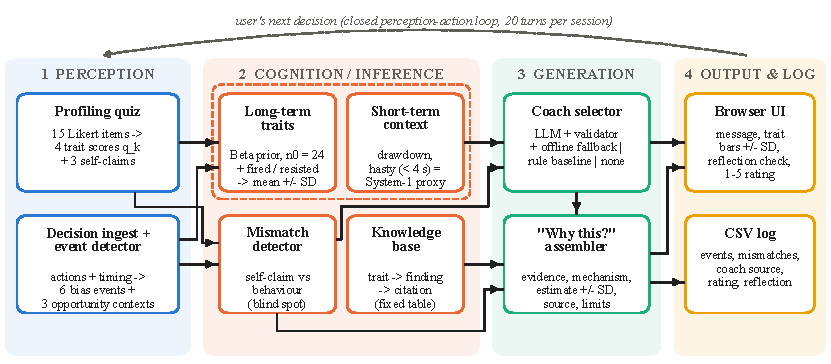
\includegraphics[width=\textwidth]{fig_architecture.pdf}
\caption{CogniFin Coach architecture. Perception turns quiz answers and decisions into trait priors, events and opportunity contexts; the dual-layer user model, mismatch detector and knowledge base perform inference; the coach generates a validated message while ``Why this?'' is assembled deterministically; the user's next decision closes the loop.}
\label{fig:arch}
\end{figure*}
Fig. 1 shows the architecture. Each of the 20 turns in a session runs a full perception--inference--generation cycle, and the user's next decision closes the loop. The four layers are described below; Algorithm 1 summarises one turn.

\subsection{Simulated environment}
Three synthetic assets follow a random walk \textit{r}\textsubscript{t} = \ensuremath{\mu} + \ensuremath{\sigma}\ensuremath{\varepsilon}\textsubscript{t} + \textit{s}\textsubscript{t}, with \ensuremath{\varepsilon}\textsubscript{t} \textasciitilde{} N(0,1), returns clipped to \ensuremath{\pm}40\%, and (\ensuremath{\mu}, \ensuremath{\sigma}) = (0.0005, 0.004) for a bond, (0.004, 0.025) for a broad index and (0.006, 0.055) for a technology fund. Scripted shocks \textit{s}\textsubscript{t} create the same decision points for every user: a rally (turns 3--5), a minor dip (8), a crash (12--13) and a recovery (15--16) (Fig. 2). A fixed seed reproduces the path exactly. Each turn the user makes one decision per asset---buy a fraction of the cash available at the start of the turn, sell a fraction of the holding, or hold---with combined buys capped at 100\% of that cash. Users may also record a reason and a 1--5 confidence rating. No real money, prices or financial data are involved.

\begin{figure}[t]
\centering
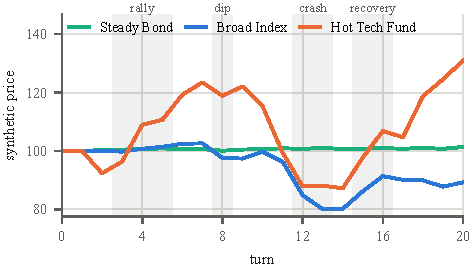
\includegraphics[width=\columnwidth]{fig_prices.pdf}
\caption{Example synthetic price path (seed 42). Shaded bands mark the scripted rally, dip, crash and recovery that every participant faces.}
\label{fig:fig_prices}
\end{figure}
\subsection{Perception layer}
\textit{Quiz.} Fifteen Likert items (1--5) are mapped to [0, 1] by (\textit{a} \ensuremath{-} 1)/4, reverse-coded where needed, and averaged into four trait scores \textit{q}\textsubscript{k} (three items each) and three self-claims: comfort with high risk, calm under loss, and trading rarely. \textit{Decisions.} For each asset decision, the event detector applies the rules in Table I to the price history, cost basis and post-trade weights. It also emits three \textit{opportunity contexts}, situations in which a bias could have shown: \texttt{dip} (holding a risky asset that fell \ensuremath{\geq} 5\% in one turn), \texttt{rally} (a risky asset up \ensuremath{\geq} 10\% over three turns while cash is available) and \texttt{loser} (holding a risky asset \ensuremath{\geq} 10\% below cost). Weaker, descriptive \textit{market-context observations} (e.g., buying after a 5\% rise) are shown and logged but never treated as evidence of a bias.

\begin{table}[t]
\caption{Behavioural event detectors and the trait each one evidences}
\centering
\footnotesize
\setlength{\tabcolsep}{3pt}
\begin{tabular}{>{\raggedright\arraybackslash}p{0.205\columnwidth}>{\raggedright\arraybackslash}p{0.521\columnwidth}>{\raggedright\arraybackslash}p{0.205\columnwidth}}
\hline
\textbf{Event} & \textbf{Trigger (prototype heuristic)} & \textbf{Trait} \\ \hline
panic\_sell & sell \ensuremath{\geq} 50\% of a holding after a \ensuremath{\geq} 5\% one-turn or \ensuremath{\geq} 7\% two-turn drop while below cost & panic selling \\
fomo\_buy & buy \ensuremath{\geq} 30\% of cash into a risky asset up \ensuremath{\geq} 10\% over three turns & herding / FOMO \\
overconc. & a buy leaves \textgreater{} 70\% of portfolio value in one risky asset & overconfidence \\
overtrading & trades on five consecutive turns & overconfidence \\
hold\_loser & keep a risky asset \ensuremath{\geq} 10\% below cost for \ensuremath{\approx} 3 turns & loss aversion \\
early\_profit & sell \ensuremath{\geq} 50\% of a \textless{} 5\% gain while holding another asset \ensuremath{\geq} 10\% below cost & loss aversion \\
\hline
\end{tabular}
\end{table}
\subsection{Long-term layer: Bayesian trait model}
For each trait \textit{k} we treat the probability \ensuremath{\theta}\textsubscript{k} that the bias is expressed, given an opportunity, as a Beta-distributed belief. The quiz supplies the prior mean and the behavioural record supplies Bernoulli evidence:

\begin{equation}
\theta_k \sim \mathrm{Beta}\big(n_0 q_k + F_k,\; n_0 (1-q_k) + R_k\big)
\end{equation}
where \textit{F}\textsubscript{k} counts turns in which an event of trait \textit{k} fired and \textit{R}\textsubscript{k} counts turns that offered the matching opportunity context but in which the bias did not fire. A turn contributes at most one trial per trait. The estimate shown to the user and passed to the coach is the posterior mean, and its uncertainty is the posterior standard deviation:

\begin{equation}
\hat\theta_k = \frac{a_k}{a_k+b_k}, \qquad \mathrm{sd}_k = \sqrt{\frac{a_k b_k}{(a_k+b_k)^2 (a_k+b_k+1)}}
\end{equation}
\textit{Prior strength.} Rather than tune \textit{n}\textsubscript{0}, we derive it from the instrument. With per-item noise of about 0.17 on the unit scale, a three-item mean has a standard error near 0.10. A Beta prior with that standard deviation at mean 0.5 has \textit{n}\textsubscript{0} = \textit{q}(1 \ensuremath{-} \textit{q})/SE\textsuperscript{2} \ensuremath{-} 1 \ensuremath{\approx} 24 pseudo-observations, so the quiz counts as much as 24 behavioural opportunities.

\textit{Why opportunities matter.} Event types have very different base rates. Across our simulated sessions a FOMO buy fires 2.64 times per session but an early profit-take only 0.04 times. The original prototype added 0.15(1 \ensuremath{-} \ensuremath{\theta}) whenever an event fired. Without a count of opportunities, that rule treats frequent detectors as strong evidence and inflates their traits, which harmed accuracy (Section IV-B). Counting fired-versus-resisted trials corrects this and yields a principled uncertainty.

\textit{Asymmetric evidence.} Overconfidence has no well-defined resisted opportunity, since any turn could be an overconfident one. Treating every turn or every trade as a trial made the estimate collapse towards zero in pilot runs, so overtrading and over-concentration contribute confirming evidence only. \textit{Persistence.} A completed session saves (\textit{F}\textsubscript{k}, \textit{R}\textsubscript{k}); the next session builds a fresh prior from a new quiz and carries the old evidence over with a forgetting factor \ensuremath{\gamma} = 0.5. Estimates map to \textit{high} (\ensuremath{\geq} 0.67), \textit{moderate} (\ensuremath{\geq} 0.40) or \textit{low} intensity labels for the coach.

\subsection{Short-term layer}
The short-term layer holds the current drawdown from the session's portfolio peak, whether the last decision was hasty (latency \textless{} 4 s), and the last five event types. It conditions the message---e.g., the coach notes that a quick decision after a fall makes gut reactions more likely---but never changes the long-term traits, so a single stressful turn cannot rewrite the profile.

\subsection{Metacognitive grounding: mismatch detector}
Because self-report is vulnerable to the bias blind spot~\cite{pronin02}, the system checks claims against behaviour. A panic sale by a user who claimed high risk tolerance or calm under loss (self-claim \ensuremath{\geq} 0.7), overtrading by a user who claimed to trade rarely, a FOMO buy by a user whose quiz herding score was \ensuremath{\leq} 0.35, and over-concentration by a user whose quiz overconfidence score was \ensuremath{\leq} 0.35 each raise a mismatch. Mismatches are shown as a neutral \textit{reflection check} (``you reported that you \ldots{}, while this turn you \ldots{}''), are passed to the coach, and are logged.

\subsection{Knowledge base and coach generation}
A fixed knowledge base maps each trait to a definition, a research finding and its citations, and each event to a trait, a description of what the rule detects, and a reflection question. Three interchangeable coaches consume the same events. The \textit{rule baseline} returns one static template per event type and ignores the profile. The \textit{personalised coach} builds a structured JSON prompt containing the event and its numbers, the bias hypothesis, the intensity label of every trait, the short-term context, the estimate's uncertainty and any mismatch. A system prompt limits the reply to two or three sentences and at most 70 words, and forbids real-world advice, price predictions, security recommendations and shaming. The reply comes from Gemini 3 Flash at a low thinking level with a 1,024-token budget. A validator rejects replies that were cut off, exceed 110 words, or match forbidden patterns (e.g., ``guaranteed'', ``will recover'', ``you should buy''). On rejection or API failure (after one retry on rate-limit or overload errors), a deterministic \textit{offline generator} fills intensity-, haste- and mismatch-conditioned templates from the same inputs. Every message carries a visible source tag (\texttt{LLM} or \texttt{offline generator}) in both the UI and the log. Because identical prompts repeated every turn habituate and lose salience, the same (event, asset) pair is not re-coached within three turns; the event is still logged and still updates the user model. A third mode, \textit{none}, is the control, and a \textit{random} mode assigns an arm for studies.

\textit{``Why this?''.} The explanation panel is assembled entirely by code. It contains what the rule noticed (in the user's own numbers), the mechanism and definition, the quiz score and current estimate \ensuremath{\pm} SD with the number of opportunities observed, session context, the research finding and citation, a reflection question, and an explicit statement of the inference's limits. The LLM never sees or writes the citation. Following Miller~\cite{miller19}, the panel is contrastive (claim versus action) and selective (one hypothesis per event, at most two prompts per turn).

\begin{figure}[t]
\centering
\fbox{\begin{minipage}{0.95\columnwidth}
\footnotesize\textbf{Algorithm 1: One turn of the CogniFin loop}\\[2pt]
{\scriptsize 1:}\hspace{0.6em}\textbf{input:} decisions \textit{D} (one per asset), latency \textit{t}, prices, portfolio, model \textit{M}\\
{\scriptsize 2:}\hspace{0.6em}events \textit{E} \ensuremath{\leftarrow} \{\};  contexts \textit{C} \ensuremath{\leftarrow} \{\};  cash\textsubscript{0} \ensuremath{\leftarrow} cash\\
{\scriptsize 3:}\hspace{0.6em}\textbf{for each} decision \textit{d} in \textit{D} \textbf{do}\\
{\scriptsize 4:}\hspace{1.8em}(\textit{e}, \textit{c}) \ensuremath{\leftarrow} DETECT(prices, portfolio, \textit{d}, history)\\
{\scriptsize 5:}\hspace{1.8em}add \textit{e} to \textit{E};  add \textit{c} to \textit{C};  apply \textit{d} using cash\textsubscript{0}\\
{\scriptsize 6:}\hspace{0.6em}update drawdown; \textit{M}.short \ensuremath{\leftarrow} (drawdown, \textit{t} \textless{} 4 s, last 5 events)\\
{\scriptsize 7:}\hspace{0.6em}\textit{X} \ensuremath{\leftarrow} MISMATCH(\textit{M}.claims, \textit{M}.quiz, \textit{E})\\
{\scriptsize 8:}\hspace{0.6em}\textbf{for each} trait \textit{k}: \textit{F}\textsubscript{k} += 1 if \textit{k} fired; \textit{R}\textsubscript{k} += 1 if ctx\textsubscript{k} in \textit{C} and not fired\\
{\scriptsize 9:}\hspace{0.6em}\textbf{for each} \textit{e} in the first two events of \textit{E} \textbf{do}\\
{\scriptsize 10:}\hspace{1.8em}msg \ensuremath{\leftarrow} COACH\textsubscript{mode}(\textit{e}, \textit{M}, \textit{X});  why \ensuremath{\leftarrow} KB(\textit{e}, \textit{M}, \textit{X})\\
{\scriptsize 11:}\hspace{0.6em}log row; render messages, reflection checks, trait bars \ensuremath{\pm} SD\\
\end{minipage}}
\end{figure}
\subsection{Implementation}
The system is about 1,650 lines of Python using only the standard library: an HTTP server with a single-page browser UI, in-memory sessions, JSON profiles and CSV interaction logs. Every row records the per-asset actions, latency, portfolio value, drawdown, events, mismatch codes, coach source and message, the user's 1--5 rating of ``did this match how you were thinking?'', and the optional reason and confidence. Thirty-nine automated tests cover detection, scoring, the Bayesian update, persistence, the coaching cooldown, LLM response handling, retry and model fallback, the HTTP API (incl. the demo seed) and the evaluation metrics.

\section{Experiments and Evaluation}
\subsection{Setup: simulated personas}
No human study has been run yet, so we evaluate the pipeline with 300 simulated personas (seed 7). Each persona has latent traits \ensuremath{\theta} \textasciitilde{} Beta(2, 2). Forty percent are ``mismatch-prone'': their panic-selling trait is at least 0.6, yet they claim high risk tolerance and calm (\ensuremath{\geq} 0.75). Quiz answers are the latent value plus N(0, 0.17) noise per item, rounded to the Likert scale. A second \textit{blind-spot} condition subtracts a persona-specific U(0, 0.35) from every trait before answering, modelling under-reported bias~\cite{pronin02}. The policy expresses traits stochastically. On a \ensuremath{\geq} 5\% dip a persona panic-sells with probability 0.95\ensuremath{\theta}\textsubscript{ps}; on a rally it buys with probability 0.9\ensuremath{\theta}\textsubscript{hf}; each turn it over-concentrates with probability 0.18\ensuremath{\theta}\textsubscript{oc} or trades with probability 0.10 + 0.55\ensuremath{\theta}\textsubscript{oc}; and it takes early profits with probability 0.5\ensuremath{\theta}\textsubscript{la}. When coached, a persona heeds the message with probability \textit{h}, suppressing the coached trait by 85\% for three turns. Coaching conditions are paired: each persona replays the same price path and noise stream in every arm. Without coaching, personas produce 6.39 bias events per session.

\textit{Caveat.} Personas are not people. The detectors and the personas share the same constructs, so detection results are optimistic upper bounds. The heed parameter is assumed, so RQ4 is a sensitivity analysis, not evidence that coaching works.

\subsection{RQ1: Trait estimation}
\begin{figure}[t]
\centering
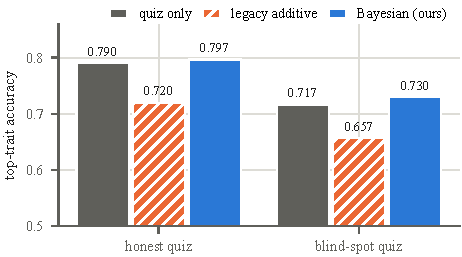
\includegraphics[width=\columnwidth]{fig_estimation.pdf}
\caption{Top-trait accuracy over 300 personas. The legacy additive rule lowers accuracy below the quiz alone; the opportunity-based Bayesian update does not, and helps when the quiz under-reports bias.}
\label{fig:fig_estimation}
\end{figure}
We compare the quiz alone, the legacy additive update and the Bayesian update on two metrics: top-trait accuracy (does the highest estimate identify the persona's strongest latent trait?) and mean absolute error over all traits (Fig. 3, Table II). With an honest quiz the legacy rule \textit{reduced} accuracy from 0.790 to 0.720, while the Bayesian update kept it at 0.797 and lowered MAE from 0.078 to 0.076. Under the blind-spot quiz, behavioural evidence becomes valuable: the Bayesian update raised accuracy from 0.717 to 0.730 and cut MAE from 0.172 to 0.158. The legacy rule achieved a lower MAE here (0.137), but only because it inflates \textit{every} trait and so partly cancels a uniform under-report. Its ranking, the quantity the coach acts on, was the worst (0.657).

\begin{table}[t]
\caption{Trait estimation (300 personas): accuracy / MAE}
\centering
\footnotesize
\setlength{\tabcolsep}{3pt}
\begin{tabular}{>{\raggedright\arraybackslash}p{0.233\columnwidth}>{\raggedright\arraybackslash}p{0.223\columnwidth}>{\raggedright\arraybackslash}p{0.242\columnwidth}>{\raggedright\arraybackslash}p{0.233\columnwidth}}
\hline
\textbf{Quiz condition} & \textbf{Quiz only} & \textbf{Legacy additive} & \textbf{Bayesian (ours)} \\ \hline
honest & 0.790 / 0.078 & 0.720 / 0.098 & \textbf{0.797} / \textbf{0.076} \\
blind spot & 0.717 / 0.172 & 0.657 / \textbf{0.137} & \textbf{0.730} / 0.158 \\
\hline
\end{tabular}
\end{table}
Fig. 4 traces one under-reporting, panic-prone persona across three persisted sessions. The estimate rises with each panic sale and falls slightly with each resisted dip, and its band narrows. However, with only three to five opportunities per session and a 24-observation prior, it closes only a small part of the gap to the latent value: the model is stable but slow.

\begin{figure}[t]
\centering
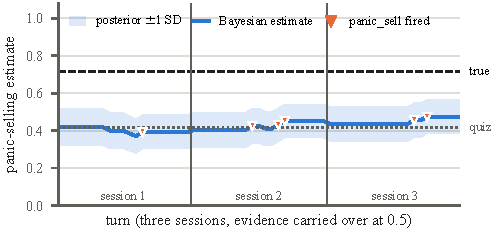
\includegraphics[width=\columnwidth]{fig_trajectory.pdf}
\caption{Panic-selling estimate (\ensuremath{\pm}1 posterior SD) for one panic-prone persona who under-reported the trait, across three sessions with evidence carried over.}
\label{fig:fig_trajectory}
\end{figure}
\subsection{RQ2: Mismatch detection}
Ground truth marks a persona as mismatched if it claims high risk tolerance (\ensuremath{\geq} 0.7) and its latent panic trait is \ensuremath{\geq} 0.6 (120 of 300). We score the two panic-related mismatch codes against this label. At the default cut-off, the detector flagged 0.91 of mismatched personas (recall) with 0.64 precision and a false-positive rate of 0.34. Requiring at least two flagged turns raises precision to 0.74 and lowers the false-positive rate to 0.12, at 0.49 recall (Fig. 5). Cut-offs of 0.6 and 0.7 give identical results, as do 0.8 and 0.9, because a single Likert item can only take the values \{0, 0.25, 0.5, 0.75, 1\}. The cut-off is effectively ordinal. Because the prompt is phrased tentatively and a false alarm costs one moment of reflection, we keep the high-recall setting for in-session prompts; any persistent label should require k \ensuremath{\geq} 2.

\begin{figure}[t]
\centering
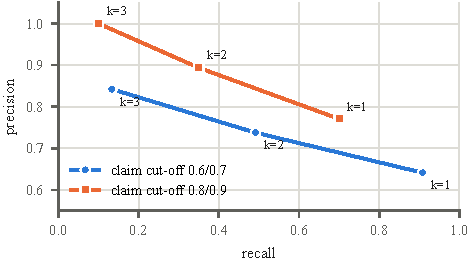
\includegraphics[width=\columnwidth]{fig_detector.pdf}
\caption{Mismatch detector precision--recall when at least k turns must be flagged, for two self-claim cut-offs.}
\label{fig:fig_detector}
\end{figure}
\subsection{RQ3: Message grounding versus a rule baseline}
We generated messages for 24 fixed scenarios (six event types \ensuremath{\times} low/high trait prior \ensuremath{\times} with/without a mismatch) from the rule baseline, the offline generator and the live LLM (Table III, Fig. 6). A message \textit{cites own numbers} if it contains a number from the event (e.g., the 15.8\% drop). Rule templates never cite the user's numbers, never use the mismatch, have no explanation panel, and produce only six distinct texts. The offline generator cited the numbers in 83\% of messages and used every supplied mismatch. The live LLM arm could not be measured at submission time: the free-tier quota and service overload (HTTP 429/503) on both models forced every call to the labelled fallback. In earlier single calls the model returned valid, grounded 50--66-word messages that cited the user's numbers and the supplied mismatch. The resumable \texttt{--llm-check} command fills in this row when quota is available. Across 415 offline-generated messages in full simulated sessions, 87\% contained the user's numbers and 100\% passed the validator. Because every explanation comes from the knowledge base, the share of hallucinated citations is zero by construction.

\begin{table}[t]
\caption{Message-level comparison on 24 fixed scenarios}
\centering
\footnotesize
\setlength{\tabcolsep}{3pt}
\begin{tabular}{>{\raggedright\arraybackslash}p{0.205\columnwidth}>{\raggedright\arraybackslash}p{0.112\columnwidth}>{\raggedright\arraybackslash}p{0.149\columnwidth}>{\raggedright\arraybackslash}p{0.121\columnwidth}>{\raggedright\arraybackslash}p{0.112\columnwidth}>{\raggedright\arraybackslash}p{0.130\columnwidth}>{\raggedright\arraybackslash}p{0.102\columnwidth}}
\hline
\textbf{Generator} & \textbf{Own nos.} & \textbf{Uses mismatch} & \textbf{Why this?} & \textbf{Words} & \textbf{Distinct} & \textbf{n} \\ \hline
rule baseline & 0\% & 0\% & 0\% & 12 & 6 & 24 \\
offline gen. & 83\% & 100\% & 100\% & 53 & 16 & 24 \\
\hline
\end{tabular}
\end{table}
\begin{figure}[t]
\centering
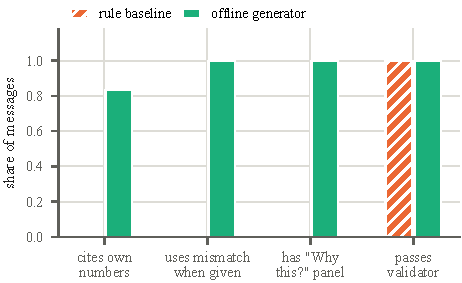
\includegraphics[width=\columnwidth]{fig_messages.pdf}
\caption{Grounding properties of the coach generators on the same 24 scenarios.}
\label{fig:fig_messages}
\end{figure}
\subsection{RQ4: Behavioural shift under assumed responsiveness}
With heed \textit{h} = 0.35 for the baseline, coaching reduced bias events from 6.39 to 6.13 per session (Fig. 7). We then let the personalised coach be heeded \ensuremath{\rho} times as often. At \ensuremath{\rho} = 1 the two coaches are identical by construction, which serves as a check of the paired design. At \ensuremath{\rho} = 1.5 the paired reduction relative to the baseline was 0.33 events [95\% bootstrap CI 0.18, 0.49], and at \ensuremath{\rho} = 2 it was 0.75 [0.53, 0.99]. The rate of repeating a coached bias within three turns fell from 0.31 to 0.25. These numbers describe the assumed model, not people. They show that personalisation pays off only to the extent that it increases how often messages are acted on---exactly the quantity a human study must measure. The persona model has no habituation, so the coaching cooldown can only shrink these simulated effects (with \texttt{COACH\_COOLDOWN\_TURNS = 0} the baseline reaches 5.77 events). Whether fewer, non-repeated prompts are heeded more often is a question the human study must answer.

\begin{figure}[t]
\centering
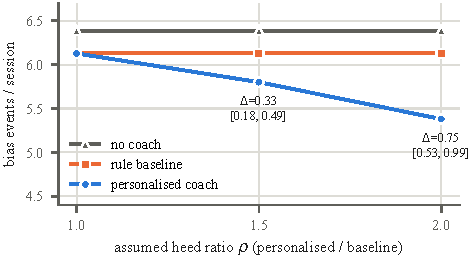
\includegraphics[width=\columnwidth]{fig_shift.pdf}
\caption{Bias events per session versus the assumed heed ratio \ensuremath{\rho}; \ensuremath{\Delta} is the paired baseline \ensuremath{-} personalised difference with a 95\% bootstrap CI.}
\label{fig:fig_shift}
\end{figure}
\subsection{Verification and QA audit}
Acting as product owner, analyst and tester, we audited the prototype against its own claims before this evaluation, and found five defects. (i) The evaluation's mismatch metric tested whether the log field was non-empty, but empty values were logged as the string ``none'', so every session counted as flagged. (ii) The mismatch ground truth covered only panic-related claims, yet it was scored against all five mismatch codes. (iii) The grounding check counted the placeholder ``no pattern detected'' as a coaching message. (iv) Gemini 3 models spend thinking tokens out of the output budget---we measured about 510--590 per reply even at the low level---so under the original 220-token cap, which also used the model's default (higher) thinking level, replies came back empty or truncated. Empty replies silently fell back to the offline generator, and truncated ones could pass the validator because the finish reason was never checked. (v) The ``losses hurt about twice as much'' claim lacked its proper source~\cite{tk92}. All five are fixed and covered by regression tests, and every number in this section was regenerated afterwards. The lesson: a fallback that is labelled in the UI can still hide a failure in aggregate metrics unless its source is logged and checked.

\section{Discussion and Future Work}
\textit{Event is not motive.} A sale after a drop may be rebalancing, and an early profit-take may reflect a liquidity need. The system therefore says ``may'', asks a reflection question, records the user's stated reason, and states its own limits in every explanation. Each event also maps to a single trait, although a panic sale can equally express loss aversion. A natural extension replaces this hard mapping with event-to-trait likelihoods in a small Bayesian network, so that one event can update several traits in proportion to how diagnostic it is.

\textit{Stability versus plasticity.} Deriving \textit{n}\textsubscript{0} from the quiz's reliability protects the profile from noisy detectors, but Fig. 4 shows the cost: learning is slow when self-report is strongly biased. Hierarchical pooling across users, opportunity-specific likelihoods, and an \textit{n}\textsubscript{0} estimated from test--retest data would let the model trust behaviour sooner when the evidence warrants it. The confirming-only evidence for overconfidence drifts upward over long horizons and needs a principled counterfactual opportunity.

\textit{Instrument and thresholds.} The quiz has three unvalidated items per trait, the detector thresholds (5\%, 10\%, 70\%, 4 s) are hand-set, and the System-1 proxy ignores individual differences in baseline speed. Future work should calibrate items with item-response theory and learn thresholds and per-user latency baselines from data.

\textit{Simulation circularity.} Because personas are built from the same constructs as the detectors, RQ1--RQ2 verify that the pipeline is internally coherent and RQ4 bounds what personalisation could achieve. None of them shows that the coach helps people.

\textit{Language-model risks.} The validator is lexical and cannot catch subtle advice or overconfident framing. We observed the LLM stating ``suggests panic selling'' more assertively than the evidence warrants. Entailment-based checks of each message against the structured evidence, and human ratings of tone, are the next safeguards. Only structured tags---never names or logs---are sent to the API.

\textit{Edge cases handled.} Buying with zero cash, selling an empty position, multiple asset decisions in one turn, over-allocated buys, duplicate assets, legacy profiles and extreme quiz answers (priors clipped to [0.01, 0.99]) are all handled and tested.

\textit{Human study.} The prototype already supports a randomised, pre-registrable study. Using the random arm (personalised, baseline or none), the primary outcome is the rate of repeated coached biases; secondary outcomes are perceived personalisation (1--5 ratings), mismatch frequency and confidence calibration. It requires ethics approval, informed consent and de-identified logs.

\section{Conclusion}
CogniFin Coach shows how a small, transparent cognitive architecture can perceive financial decisions, maintain an uncertainty-aware model of a user's biases, confront self-report with behaviour, and explain each inference without letting a language model invent its grounds. Replacing an ad-hoc additive update with an opportunity-based Bayesian model, whose prior strength follows from the instrument's reliability, turned behavioural evidence from a liability into a modest gain. The audit showed that silent fallbacks and sentinel values can invalidate an evaluation without breaking a single test. The decisive next step is a study with people.

\section*{Acknowledgment}
Prepared for CPE 663: Cognitive Computing, Term Project. Evaluation results use simulated personas only; no human-subject data were collected.

\begin{thebibliography}{99}
\bibitem{bo00} B. M. Barber and T. Odean, ``Trading is hazardous to your wealth: The common stock investment performance of individual investors,'' \textit{J. Finance}, vol. 55, no. 2, pp. 773--806, 2000.
\bibitem{ss85} H. Shefrin and M. Statman, ``The disposition to sell winners too early and ride losers too long: Theory and evidence,'' \textit{J. Finance}, vol. 40, no. 3, pp. 777--790, 1985.
\bibitem{odean98} T. Odean, ``Are investors reluctant to realize their losses?'' \textit{J. Finance}, vol. 53, no. 5, pp. 1775--1798, 1998.
\bibitem{flm14} D. Fernandes, J. G. Lynch, Jr., and R. G. Netemeyer, ``Financial literacy, financial education, and downstream financial behaviors,'' \textit{Manage. Sci.}, vol. 60, no. 8, pp. 1861--1883, 2014.
\bibitem{lm14} A. Lusardi and O. S. Mitchell, ``The economic importance of financial literacy: Theory and evidence,'' \textit{J. Econ. Literature}, vol. 52, no. 1, pp. 5--44, 2014.
\bibitem{dpr19} F. D'Acunto, N. Prabhala, and A. G. Rossi, ``The promises and pitfalls of robo-advising,'' \textit{Rev. Financial Stud.}, vol. 32, no. 5, pp. 1983--2020, 2019.
\bibitem{kahneman11} D. Kahneman, \textit{Thinking, Fast and Slow}. New York, NY, USA: Farrar, Straus and Giroux, 2011.
\bibitem{es13} J. St. B. T. Evans and K. E. Stanovich, ``Dual-process theories of higher cognition: Advancing the debate,'' \textit{Perspect. Psychol. Sci.}, vol. 8, no. 3, pp. 223--241, 2013.
\bibitem{loewenstein96} G. Loewenstein, ``Out of control: Visceral influences on behavior,'' \textit{Organ. Behav. Hum. Decis. Process.}, vol. 65, no. 3, pp. 272--292, 1996.
\bibitem{pronin02} E. Pronin, D. Y. Lin, and L. Ross, ``The bias blind spot: Perceptions of bias in self versus others,'' \textit{Pers. Soc. Psychol. Bull.}, vol. 28, no. 3, pp. 369--381, 2002.
\bibitem{fischhoff82} B. Fischhoff, ``Debiasing,'' in \textit{Judgment Under Uncertainty: Heuristics and Biases}, D. Kahneman, P. Slovic, and A. Tversky, Eds. Cambridge, U.K.: Cambridge Univ. Press, 1982, pp. 422--444.
\bibitem{larrick04} R. P. Larrick, ``Debiasing,'' in \textit{Blackwell Handbook of Judgment and Decision Making}, D. J. Koehler and N. Harvey, Eds. Oxford, U.K.: Blackwell, 2004, pp. 316--337.
\bibitem{morewedge15} C. K. Morewedge, H. Yoon, I. Scopelliti, C. W. Symborski, J. H. Korris, and K. S. Kassam, ``Debiasing decisions: Improved decision making with a single training intervention,'' \textit{Policy Insights Behav. Brain Sci.}, vol. 2, no. 1, pp. 129--140, 2015.
\bibitem{flavell79} J. H. Flavell, ``Metacognition and cognitive monitoring: A new area of cognitive--developmental inquiry,'' \textit{Amer. Psychol.}, vol. 34, no. 10, pp. 906--911, 1979.
\bibitem{kt79} D. Kahneman and A. Tversky, ``Prospect theory: An analysis of decision under risk,'' \textit{Econometrica}, vol. 47, no. 2, pp. 263--291, 1979.
\bibitem{tk92} A. Tversky and D. Kahneman, ``Advances in prospect theory: Cumulative representation of uncertainty,'' \textit{J. Risk Uncertainty}, vol. 5, no. 4, pp. 297--323, 1992.
\bibitem{bo01} B. M. Barber and T. Odean, ``Boys will be boys: Gender, overconfidence, and common stock investment,'' \textit{Q. J. Econ.}, vol. 116, no. 1, pp. 261--292, 2001.
\bibitem{banerjee92} A. V. Banerjee, ``A simple model of herd behavior,'' \textit{Q. J. Econ.}, vol. 107, no. 3, pp. 797--817, 1992.
\bibitem{bhw92} S. Bikhchandani, D. Hirshleifer, and I. Welch, ``A theory of fads, fashion, custom, and cultural change as informational cascades,'' \textit{J. Political Econ.}, vol. 100, no. 5, pp. 992--1026, 1992.
\bibitem{simon55} H. A. Simon, ``A behavioral model of rational choice,'' \textit{Q. J. Econ.}, vol. 69, no. 1, pp. 99--118, 1955.
\bibitem{actr04} J. R. Anderson, D. Bothell, M. D. Byrne, S. Douglass, C. Lebiere, and Y. Qin, ``An integrated theory of the mind,'' \textit{Psychol. Rev.}, vol. 111, no. 4, pp. 1036--1060, 2004.
\bibitem{as68} R. C. Atkinson and R. M. Shiffrin, ``Human memory: A proposed system and its control processes,'' in \textit{The Psychology of Learning and Motivation}, vol. 2, K. W. Spence and J. T. Spence, Eds. New York, NY, USA: Academic Press, 1968, pp. 89--195.
\bibitem{ca94} A. T. Corbett and J. R. Anderson, ``Knowledge tracing: Modeling the acquisition of procedural knowledge,'' \textit{User Model. User-Adapt. Interact.}, vol. 4, no. 4, pp. 253--278, 1994.
\bibitem{grossberg87} S. Grossberg, ``Competitive learning: From interactive activation to adaptive resonance,'' \textit{Cogn. Sci.}, vol. 11, no. 1, pp. 23--63, 1987.
\bibitem{ts08} R. H. Thaler and C. R. Sunstein, \textit{Nudge: Improving Decisions About Health, Wealth, and Happiness}. New Haven, CT, USA: Yale Univ. Press, 2008.
\bibitem{ji23} Z. Ji \textit{et al.}, ``Survey of hallucination in natural language generation,'' \textit{ACM Comput. Surv.}, vol. 55, no. 12, pp. 1--38, 2023.
\bibitem{lewis20} P. Lewis \textit{et al.}, ``Retrieval-augmented generation for knowledge-intensive NLP tasks,'' in \textit{Proc. Adv. Neural Inf. Process. Syst. (NeurIPS)}, vol. 33, 2020, pp. 9459--9474.
\bibitem{miller19} T. Miller, ``Explanation in artificial intelligence: Insights from the social sciences,'' \textit{Artif. Intell.}, vol. 267, pp. 1--38, 2019.
\end{thebibliography}
\appendices
\section{Code Repository and Reproduction}
\textbf{Code repository:} \url{https://github.com/AungkhinemoeLIM/cognifin-coach}

\textbf{Environment:} Python \ensuremath{\geq} 3.9 (tested on 3.13); the application uses only the standard library. \texttt{pytest} runs the tests and \texttt{matplotlib} regenerates the figures. Gemini is optional: put \texttt{GEMINI\_API\_KEY} (and optionally \texttt{COGNIFIN\_MODEL}, default \texttt{gemini-3-flash-preview}) in \texttt{.env}; without a key the labelled offline generator is used.

\begin{verbatim}
git clone https://github.com/AungkhinemoeLIM/cognifin-coach
cd cognifin-coach
pip install -r requirements.txt  # pytest, matplotlib
python app.py           # open http://localhost:8000
python -m pytest -q tests        # 39 tests
python -m cognifin.evaluate --n 300 --out results
python -m cognifin.evaluate --extra --out results
python -m cognifin.evaluate --llm-check --out results
python paper/make_figures.py && python paper/build_paper.py
\end{verbatim}
\textbf{Repository layout:} \texttt{cognifin/} (quiz, simulator, user model, mismatch, knowledge base, coaches, session, personas, evaluation), \texttt{static/} (UI), \texttt{tests/}, \texttt{results/} (evaluation outputs), \texttt{paper/} (this paper, figures, LaTeX source), \texttt{presentation/} (slides, speaker notes) and \texttt{demo/} (demonstration script).

\end{document}
